The following Definitions are particular instances of the extremely general formulations of those in \cite{Mazzola} which carry the same name. The full generality is avoided here due to our underlying agenda: to relate musical composition to computation. The indications of such a relationship described in the Introduction encourage us to look toward \emph{global compositions}, which consist of a collection of particular \emph{local compositions}, satisfying suitable compatibility conditions. Our approach avoids the full generality of \emph{forms} and avoids \emph{denotators} completely, which greatly reduces the work needed to arrive at \emph{global compositions}.\\\\
%
First we Define \emph{forms}, we differ from Mazzola's recursive Definition and provide an inductive one instead, throughout rings are assumed to be commutative with unit.
\begin{defn}
 The set of \textbf{simple forms} $\scr{F}$ consists of tuples $(N(F),T(F),C(F),I(F))$ where
 \begin{itemize}
  \item the \textbf{name} $N(F)$ is a word in $\operatorname{ASCII}^\ast$,
  \item the \textbf{type} $T(F)$ is the word $\operatorname{Simple} \in \operatorname{ASCII}^\ast$,
  \item the \textbf{coordinator} is a ring $R$ along with an $R$-module $M$,
  \item the \textbf{identifier} $I(F)$ is a presheaf $S: \underline{Modd}^{\text{op}} \to \underline{Set}$ along with a monic $S \rightarrowtail \underline{Modd}(\und{0.2},M)$.
 \end{itemize}
 We now define \textbf{compound forms}, let $i > 0$ and $N(F) \in \operatorname{ASCII}^\ast$,
 \begin{itemize}
  \item if $(F' = N(F'), T(F'), C(F'), I(F')) \in \scr{F}_{i - 1}$, then
  \begin{itemize}
   \item if $I(F): X \to \operatorname{Dom}I(F')$ is some monic of functors, then $F = (N(F), \operatorname{Syn}, F', I(F)) \in \scr{F}_{i}$, we say $F$ has type \textbf{synonym},
   \item if $I(F): X \to \Omega^{\operatorname{Dom}I(F')}$ is some monic of functors, then $F = (N(F), \operatorname{power}, F', I(F)) \in \scr{F}_i$, we say $F$ has type \textbf{Power}
  \end{itemize}
    \item given a diagram $D: \scr{J} \to \underline{Set}^{\underline{Modd}^{op}}$ and a $\scr{J}$-indexed collection $\lbrace F_j: (N(F_j),T(F_j), C(F_j), I(F_j))\rbrace_{j \in J}$ where $F_j \in \scr{F}_{i-1}$ and $D(j) = \operatorname{Dom}I(F_j)$ then
    \begin{itemize}
     \item $F = (N(F), \operatorname{Limit}, D, \operatorname{Limit}_{D}\scr{J}) \in \scr{F}_j$, we say $F$ has type \textbf{limit}, and
     \item $F = (N(F), \operatorname{Colimit}, D, \operatorname{Colimit}_D\scr{J}) \in \scr{F}_j$, we say $F$ has type \textbf{colimit}.
    \end{itemize}
 \end{itemize}
As with simple forms, the \textbf{name} of a compound form $F = (N(F), T(F), C(F), I(F))$ is $N(F)$, etc.
\end{defn}
\begin{example}
\label{OnsetPitch}
 An extremely bare bones way of thinking about a musical phrase played by a musician is as a sequence of notes. Assuming these notes belong to the standard $12$-tone equal temprament tuning, and are played on a monophonic instrument, this can be formalised as a sequence of elements of the $\bb{Z}$-module $\bb{Z}_m \oplus \bb{Z}_{12}$, where $m$ is the length of the sequence. An element $(a,b)$ means the $a^\text{th}$ note in the music phrase is that which is $b$ semitones above $C$. That is, $\bb{Z}_m$ determines the \emph{onset} of the note, and $\bb{Z}_{12}$ determins the \emph{pitch}. This data is captured by the following form:
 \[(\operatorname{OnsetPitch}_{(m,12)},\operatorname{Simple}, \bb{Z}_m\oplus\bb{Z}_{12},\operatorname{Id}_{y(\bb{Z}_m\oplus\bb{Z}_{12})})\]
 where $y: \underline{Modd} \to \underline{Set}^{\underline{Modd}^{\text{op}}}$ is the Yoneda embedding.
\end{example}
\begin{remark}
 At this point, the roll of the identifier of a form may seem like an illusive concept, especially since the only Example given here is so trivial. Indeed the full weight of the abstract setting will not be needed for our current purposes, in fact the identifier can safely be completely ignored for the remainder of this note. It was included in order to align with \cite{Mazzola}. See \cite[p.56]{Mazzola} for the motivation for having it as part of the Definition of a form.
\end{remark}
\begin{defn}
 Let $R$ be a ring
 \label{localcompositions}and $M$ and $R$-module. An \textbf{$M$ addressed local composition} $\call{C}$ is a tuple $(N(\call{C}), F,X)$ where
 \begin{itemize}
  \item $N(\call{C})$ is a name, that is, a word in $\operatorname{ASCII}^\ast$,
  \item $F$ is a form,
  \item $X$ is a subset of $\operatorname{Dom}I(F)(M)$
 \end{itemize}
\end{defn}
\begin{remark}
 The corresponding notion to \ref{localcompositions} in \cite{Mazzola} is \emph{objective local compositions}, see \cite[\S7, p90]{Mazzola}.
\end{remark}
\begin{defn}
 A \textbf{morphism} of $M$ addressed local compositions $f:(N,F_N,X)\to (P,F_P,Y)$ is a function $f: X \to Y$ such that there exists a natural transformation $\eta: \operatorname{Dom}I(F_N) \to \operatorname{Dom}I(F_P)$ such that the following diagram commutes
 \[
  \begin{tikzcd}
   X\arrow[r,rightarrowtail]\arrow[d,swap,"f"] &\operatorname{Dom}I(F_N)(M)\arrow[d,"{h_M}"]\\
   Y\arrow[r,rightarrowtail]&\operatorname{Dom}I(F_P)(M)
  \end{tikzcd}
 \]
\end{defn}
Local compositions can be \emph{glued together} to form \emph{global compositions}:
\begin{defn}
 Let $R$ be a ring and $M$ an $R$-module. A \textbf{$M$ addressed pre-global composition} consists of the following data:
 \begin{itemize}
  \item a set $G$,
  \item a non-empty covering $\lbrace I_j \rbrace_{j \in J}$ of $G$,
  \item an \textbf{$M$ addressed atlas} for the covering $I$ of $G$, which consists of
  \begin{itemize}
   \item a family $\lbrace \call{C}_t = (N(\call{C}_t),F_t,X_t)\rbrace_{t \in T}$ of $M$ addressed local compositions,
   \item a surjection $s: T \twoheadrightarrow J$, we write $I_t$ for $I_{s(t)}$,
   \item for each $t \in T$, a bijection $\phi_t: X_t \stackrel{\sim}{\longrightarrow}I_t$
  \end{itemize}
such that if $I_t \cap I_{t'} \neq \varnothing$, we have that $\phi_t: \phi_t^{-1}(I_t \cap I_{t'}) \to \phi_{t'}^{-1}(I_t \cap I_{t'})$ is part of an isomorphism of local compositions $\call{C}_t \stackrel{\sim}{\to}\call{C}_{t'}$.
 \end{itemize}
Two $M$ addressed atlases for the covering $I$ of $G$ are \textbf{equivalent} if their disjoint union is again an $M$ addressed atlas for the covering $I$ of $G$. Two $M$ addressed pre-global compositions are \textbf{equivalent} if their $M$ addressed atlases for the covering $I$ of $G$ are equivalent. An \textbf{$M$ addressed global composition} is an equivalence class of $M$ addressed pre-global compositions.
\end{defn}
\begin{example}
 See Figure \ref{Boulez} for a musical phrase consisting of 12 notes. The set $G$ is this collection of notes, and the covering are the labelled squares. The address is the zero-module, and all 15 local compositions have associated form given by $\operatorname{OnsetPitch_{(0,12)}}$. This is included here only to provide rough intuition. See \cite[\S13.2]{Mazzola} for details.
 \begin{figure}[h]
 \centering
 \label{Boulez}
 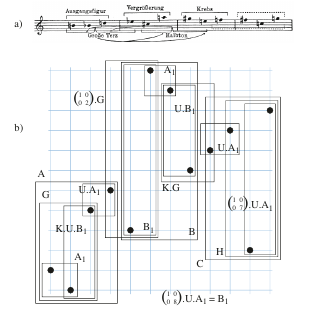
\includegraphics[width = 10cm]{Pictures/Boulez.png}
 \caption{A global composition}
\end{figure}
\end{example}
\begin{defn}
\label{nerve}
 The \textbf{nerve} of an $M$ addressed global composition is the categorical nerve of the covering $I$ of $G$ which is a poset thought of as a category.
\end{defn}
\begin{remark}
 Definition \ref{nerve} differs from the notion with the same name is \cite{Mazzola}, there, the nerve is taken as a simplicial complex rather than a simplicial set.
\end{remark}
\begin{lemma}
 The Geometric realisation of the nerve of a global composition gives the nerve as defined in \cite[\S13.2.1]{Mazzola}.
\end{lemma}
\begin{remark}
 There exists an appropriate notion of \emph{morphism} of global compositions which together with global compositions themselves form a category, and moreover the nerve can be extended to a functor from this category to the homotopy category of simplicial sets. See \cite[\S13,\S14]{Mazzola} for details. This provides a way to inject homotopy theory into musicology, and provides a way to derive topological and therefor algebraic invariants of global compositions. This is not the direction this note will take though.
\end{remark}
This leads us to the following question:
\begin{question}
 If global compositions are simplicial sets, then how can they be related to something ``computational'', or ``algorithmic''?
\end{question}
Another unfinished project, that (finite) simplicial sets are algorithms \cite{simsetsarealgs} may be relevant here.\\\\
%
Also, music plays from start to finish, so the local compositions ``pan from left to right'' in some sense, that is, they play out in \emph{order} from left to right, but with overlap due to that of the charts of the global composition. These charts when thought of as \emph{transitions} from one \emph{musical element} $\tau$ to another $\sigma$ appear strikingly similar to a $\lambda$-term of type $\tau \to \sigma$. However, as we have just seen, global compositions are not $\lambda$-terms, they are simplicial sets. So a mathematical question arises:
\begin{question}
 Is there any circumstance in which a simplicial set can be described by a typed $\lambda$-term?
\end{question}
A positive answer to this question would be ``yes, when that simplicial set arrises from a global composition''. Fleshing out the details of such an answer would then lead to a result similar to the \emph{curry-howard correspondence} \cite{MurfetTroiani} which extends the ``types as propositions, terms as proofs'' paradigm to ``types as propositions as musical elements, terms as proofs as compositions'' paradigm. A holy grail in this search would be a new perspective which renders mathematical musicology relevant to computer science, in the same way that insights of the 1950s and 1960s rendered proof theory relevant to computer science.\\\\
%
Notice also that with careful construction of the notion of ``musical element'', there could be collections of ``musical elements'' of particular sorts, for example, a local composition $\call{C}$ which starts on a $C$ and a local composition $\call{C}$ which starts on $G$ are both ``musical elements'' of sort ``belong to the $C$-major scale''. So perhaps even System F is the appropriate computational model for global compositions.

































